\problemname{Carnival General}
Every four years, the students of Lund come together to organize the Lund Carnival. For a few days, 
a park fills with tents where all kinds of festive activities take place.
The person in charge of making this happen is the carnival general. 

In total, there have been $N$ carnivals, each with a different general. The generals are numbered
from $0$ to $N-1$ in chronological order. Every general $i$ has given their opinion on how good
their predecessors were, by publishing a ranking of the generals $0, 1, \ldots, i-1$
in order from best to worst.

The next Lund Carnival will be in 2026. In the meantime, all past carnival generals have 
gathered to take a group photo. However, it would be awkward if generals $i$ and $j$ (where $i < j)$
end up next to each other if $i$ is \textbf{strictly} in the second half of $j$'s ranking.

For example:

\begin{itemize}
  \item If general $4$ has given the ranking \verb|3 2 1 0|, then $4$ can stand next to $3$, or $2$, but not $1$ or $0$.
  \item If general $5$ has given the ranking \verb|4 3 2 1 0|, then $5$ can stand next to $4, 3$ or $2$, but not $1$ or $0$.
\end{itemize}

Note that it is fine if one general is exactly in the middle of another's ranking. 

The following figure illustrates sample 1. Here, general $5$ stands next to generals $2$ and $3$, 
and general $4$ stands next to general $2$ only.

\begin{center}
  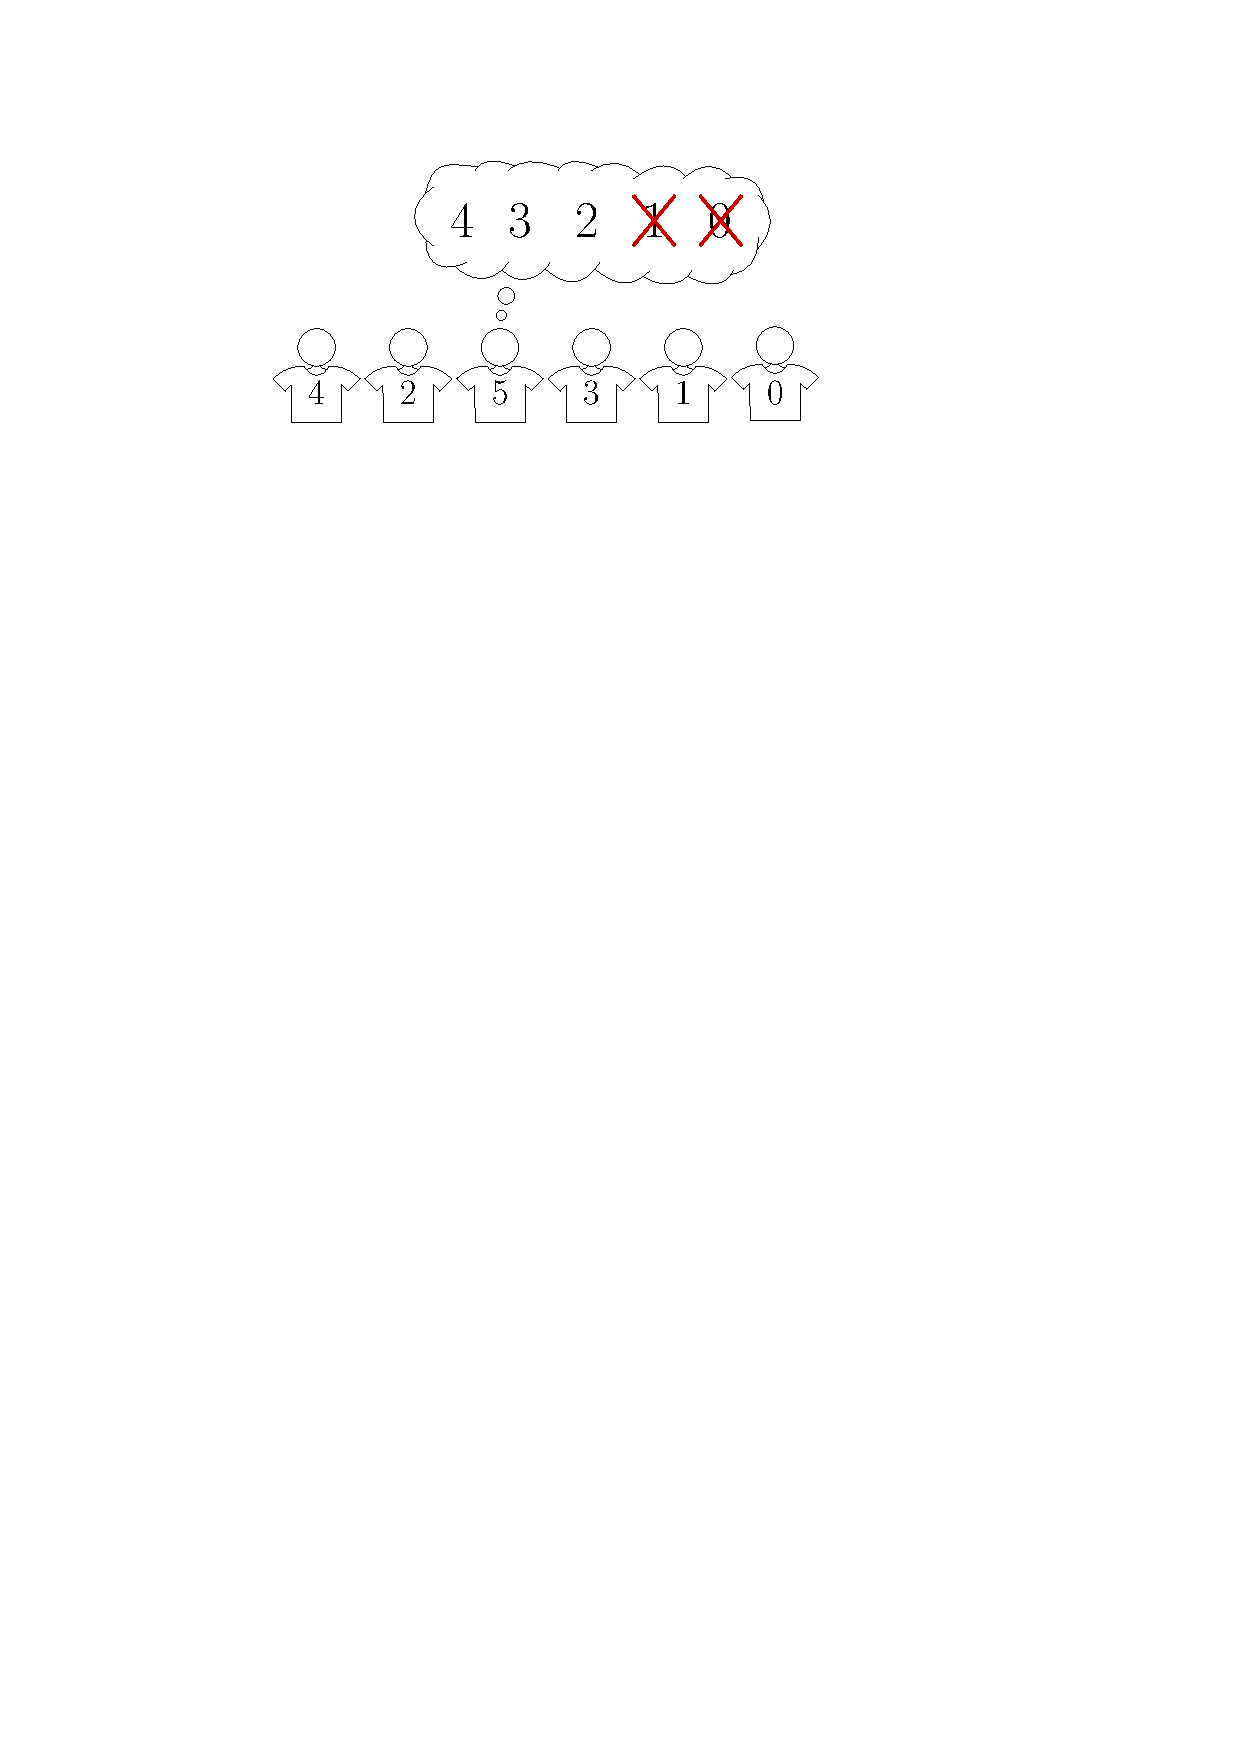
\includegraphics[width=.8\textwidth]{sample}
\end{center}


You are given the rankings that the generals published. 
Your task is to arrange the generals $0,1,\ldots, N-1$ in a row, so that if $i$ and $j$ are adjacent 
(where $i < j$) then $i$ is \textbf{not} strictly in the second half of $j$'s ranking.


\section*{Input}

The first line contains the positive integer $N$, the number of generals.

The following $N-1$ lines contain the rankings. 
The first of these lines contains general $1$'s ranking, the second line contains general $2$'s ranking, 
and so on until general $N-1$. General $0$ is absent since general $0$ didn't have any predecessors to rank.

The ranking of general $i$ is a list with $i$ integers $p_{i,0}, p_{i,1}, \ldots, p_{i,i-1}$ 
in which every integer from $0$ to $i-1$ occurs exactly once.
Specifically, $p_{i,0}$ is the best and $p_{i,i-1}$ is the worst general according to general $i$.


\section*{Output}

Print a list of integers, an ordering of the numbers $0, 1, \ldots, N-1$, such that for each pair of adjacent numbers, 
neither is strictly in the second half of the other's ranking.

It can be proven that a solution always exists.
If there are multiple solutions, you may print any of them.

\section*{Constraints and Scoring}

\noindent
\begin{itemize}
  \item $2 \leq N \leq 1000$.
  \item $0 \leq p_{i,0}, p_{i,1}, \ldots, p_{i,i-1} \leq i-1$ for $i = 0, 1, \ldots, N-1$.
\end{itemize}


Your solution will be tested on a set of test groups, each worth a number of points. 
Each test group contains a set of test cases. To get the points for a test group you need to 
solve all test cases in the test group.

\noindent
\begin{tabular}{| l | l | l |}
\hline
Group & Score & Limits \\ \hline
  1      & 11      & The ranking of general $i$ will be $i-1, i-2, \ldots, 0$ for all $i$ such that $1 \leq i \leq N-1$ \\ \hline
  2      & 23      & The ranking of general $i$ will be $0, 1, \ldots, i-1$ for all $i$ such that $1 \leq i \leq N-1$  \\ \hline
  3      & 29      & $N \leq 8$  \\ \hline
  4      & 37      & No additional constraints  \\ \hline
\end{tabular}

\section*{Example}

The first sample matches the condition of test group $1$. 
In this sample, neither general $2$ nor $3$ can stand next to general $0$, and neither general $4$ nor $5$ 
can stand next to generals $0$ and $1$. The sample output was illustrated in the figure above.

The second sample matches the condition of test group $2$. 
In this sample, general $2$ can't stand next to general $1$, general $3$ can't stand next to general $2$, 
and general $4$ can't stand next to generals $3$ and $2$.

The third sample matches the condition of test group $3$. 
In this sample, the only pairs of generals that can't stand next to each other are $(1, 3)$ and $(0, 2)$.
Hence, there are no conflicts if they are arranged \verb|3 0 1 2|. Another possible answer is \verb|0 1 2 3|.
